\documentclass[11pt,a4paper]{article}

\usepackage{epsfig}
\usepackage{multicol}

\usepackage[utf8]{inputenc}
\usepackage[brazil]{babel}
\usepackage{fancyheadings}
\usepackage{amsmath}
\usepackage{calrsfs}
\usepackage{enumerate}
\usepackage{enumitem}   
\DeclareGraphicsExtensions{.png,.pdf}
\usepackage{amsmath, amsfonts, amssymb}
\usepackage{esint}
\usepackage{graphicx}
\usepackage{multicol}
\usepackage{tasks}
\usepackage[utf8]{inputenc}
\usepackage{mathrsfs} % Transformada de Laplace
\usepackage{indentfirst}
\usepackage{xcolor}

% As margens
\setlength{\textheight}{24.0cm}
\setlength{\textwidth}{17.5cm}
\setlength{\oddsidemargin}{2.0cm} % Margens reais desejadas
\setlength{\evensidemargin}{2.0cm} % 2+17.5+1.5=21cm (largura A4)
\setlength{\topmargin}{1.5cm} % 1.5+1.6+1.0+24.0+1.6=29.7cm
\setlength{\headheight}{1.6cm} % (altura A4)
\setlength{\headsep}{1.0cm}
\setlength{\columnsep}{1.5cm} % Coluna = 8cm ((17.5-1.5)/2)
\addtolength{\oddsidemargin}{-1in}
\addtolength{\evensidemargin}{-1in}
\addtolength{\topmargin}{-1in}
\setlength{\footskip}{0.0cm}


% Novos comandos
\newcommand{\limite}{\displaystyle\lim}
\newcommand{\integral}{\displaystyle\int}
\newcommand{\somatorio}{\displaystyle\sum}
\newcommand{\mat}[1]{\mbox{\boldmath{$#1$}}} 

\pagestyle{fancy}


\usepackage{lipsum}

\lhead{

\includegraphics[width=1cm]{brasao.png}
}

\rhead{ 
\sc\textbf{U}niversidade \textbf{F}ederal do \textbf{C}eará\\
Campus Quixadá\\ Lista 6 de Eletromagnetismo}

\cfoot{}

\begin{document}

	\begin{center}
		\Large Eletrodinâmica - Corrente elétrica, Lei de Ohm e Força eletromotriz (fem). 
	\end{center}

\begin{flushleft}
\textbf{Nome:} Mateus Sousa Araújo. \\
\textbf{Matrícula:} 374858. \\
\textbf{Professor:} Antônio Joel Ramiro de Castro. \\
\textbf{Curso:} Engenharia de Computação. \\
\end{flushleft}

\begin{enumerate}

\item \textbf{Griffiths - Cap. 7 - Problema 7.1.}

Duas cascas de metal, esféricas e concêntricas, de raios $a$ e $b$, respectivamente, são separadas por material condutir, de condutividade $\sigma$.

\begin{figure}[h]	
\centering % para centralizarmos a figura	
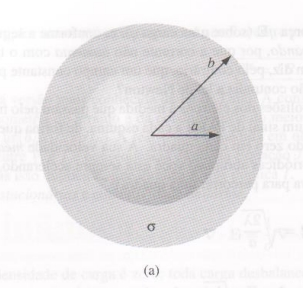
\includegraphics[width=5cm]{Selection_092.jpg} 
\end{figure}

\begin{enumerate}
\item Se elas forem mantidas a uma diferença de potencial $V$, que corrente passará de uma para a outra?
\item Qual é a resistência entre as cascas?
\item Observe que se $b>>a$ o raio externo $(b)$ é irrelevante. Como você explica isso? Explore esta observação para determinar a corrente que passa entre duas esferas de metal, ambas de raio $a$, mergulhadas no fundo do mar e mantidas a uma grande distância uma da outra, se a diferença de potencial entre elas é $V$. (Esse arranjo pode ser usado para medir a condutividade da água do mar.)

\begin{figure}[h]	
\centering % para centralizarmos a figura	
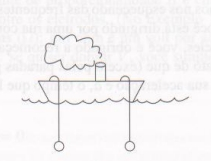
\includegraphics[width=4cm]{Selection_093.jpg} 
\end{figure}
\end{enumerate}


\textbf{RESOLUÇÃO}

\begin{enumerate}

\item 

Sendo $Q$ a carga interna da esfera menor, temos que o campo entre as duas é dado por:

$$E = \displaystyle\dfrac{1}{4\pi \epsilon_0} \displaystyle\dfrac{Q}{r^2}$$

A diferença de potencial pode ser escrito na seguinte forma:

$$(V_a - V_b) = -\displaystyle\int_b^{a} E \cdot dr = -\displaystyle\dfrac{1}{4\pi \epsilon_0} Q \displaystyle\int_b^{a} \displaystyle\dfrac{1}{r^2} \ dr$$

$$(V_a - V_b) = \displaystyle\dfrac{1}{4\pi \epsilon_0}\left(\displaystyle\dfrac{1}{a} - \displaystyle\dfrac{1}{b}\right)$$

Por definição temos:

$$I = \displaystyle\int J \cdot da = \sigma\displaystyle\int E \cdot da = \sigma \displaystyle\dfrac{Q}{\epsilon_0} = \displaystyle\dfrac{\sigma}{\epsilon_0} \displaystyle\dfrac{4\pi \epsilon_0 (V_a - V_b)}{1/a - 1/b} = 4\pi\sigma \displaystyle\dfrac{(V_a - V_b)}{1/a - 1/b}$$

\item

Usando a Lei de Ohm, temos:

$$R = \displaystyle\dfrac{V_a - V_b}{I} = \displaystyle\dfrac{1}{4\pi \epsilon_0} \left(\displaystyle\dfrac{1}{a} - \displaystyle\dfrac{1}{b}\right)$$ 

\item

Para um raio $b$ muito grande o segundo termo é desprezível, logo:

$$R = \displaystyle\dfrac{1}{4\pi \sigma a}$$

A resistência se apresenta na região em torno da esfera menor. Para duas esferas submersas, temos:

$$R = \displaystyle\dfrac{1}{2\pi \sigma a}$$

Usando a lei de Ohm, temos que a corrente é:

$$I = \displaystyle\dfrac{V}{R} = 2\pi \sigma a V$$

\end{enumerate}


\item \textbf{Griffiths - Cap. 7 - Problema 7.5.}


Uma bateria de fem $\varepsilon$ e resistência interna $r$ está ligada a uma resistência de 'carga' variável $R$. Se você quiser fornecer o máximo possível de potência para a resistência de 'carga', que resistência $R$ deve escolher? (Você não pode, é claro, alterar $\varepsilon$ e $r$.)

\textbf{RESOLUÇÃO}

Considerando que a resistência interna $r$ está em série com a carga, temos que a corrente é:

$$I = \displaystyle\dfrac{\varepsilon}{r + R}$$

O cálculo da potência é dado por:

$$P = I^2R$$

Substituindo a corrente $I$ do circuito na expressão acima, temos:

$$P = \displaystyle\dfrac{\varepsilon^2R}{(r + R)^2}$$

Se quisermos fornecer potência máxima, precisamos derivar a equação acima em relação a $R$ e igualar a zero. Dessa forma, temos:

$$\displaystyle\dfrac{dP}{dR} = \varepsilon^2\left[\displaystyle\dfrac{1}{(r + R)^2} - \displaystyle\dfrac{2R}{(r + R)^3}\right] = 0$$

Simplificando a expressão acima, temos:

$$r + R = 2R$$

$$R = r$$

Devemos ajustar a resistência interna do gerador como sendo igual a resistência da carga ou vice-versa. Dessa forma, forneceremos uma potência máxima a essa carga.

\item \textbf{Griffiths - Cap.7 - Problema 7.6.}

Uma espira retangular de fio está situada de forma que uma extremidade (altura h) fica entre as placas de um capacitor de placas paralelas, com orientação paralela ao campo $E$. A outra extremidade fica bem fora, onde o campo é essencialmente nulo. Qual é a fem dessa espira? Se a resistência total é $R$, que corrente passa? Explique. [Alerta: esta é uma pergunta capciosa, portanto tenha cuidado; se você inventou uma máquina de moto-perpétuo, ela provavelmente tem algum problema.]

\begin{figure}[h]	
\centering % para centralizarmos a figura	
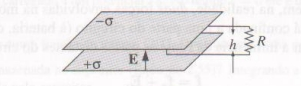
\includegraphics[width=5cm]{Selection_094.jpg} 
\end{figure}



\textbf{RESOLUÇÃO}

Considerando a expressão

$$\varepsilon = \displaystyle\oint E \cdot dl$$

Podemos concluir que a fem de um campo elétrico conservativo é sempre zero. Além disso, a integral num caminho fechado em um campo conservativo, como é o caso da questão acima, também é zero. O campo gerado entre as placas de um capacitor é de origem eletrostática. Por esse motivo, a fem sempre será igual a zero.



\end{enumerate}
	
\end{document}